% Created 2020-05-27 Wed 10:43
% Intended LaTeX compiler: lualatex
\documentclass[a4paper,12pt,twoside]{report}
\usepackage{graphicx}
\usepackage{grffile}
\usepackage{longtable}
\usepackage{wrapfig}
\usepackage{rotating}
\usepackage[normalem]{ulem}
\usepackage{amsmath}
\usepackage{textcomp}
\usepackage{amssymb}
\usepackage{capt-of}
\usepackage{hyperref}
\usepackage{color}
\usepackage{listings}
\usepackage[a4paper,margin=1cm]{geometry}
\author{Vladimir Nikishkin}
\date{\today}
\title{Exercise 3.9 Environment structures}
\hypersetup{
 pdfauthor={Vladimir Nikishkin},
 pdftitle={Exercise 3.9 Environment structures},
 pdfkeywords={},
 pdfsubject={},
 pdfcreator={Emacs 26.3 (Org mode 9.3.4)}, 
 pdflang={English}}
\begin{document}

\maketitle
\tableofcontents

Okay, this is not a very good solution. I only display the
environments, and the code is only displayed to clarify the
environments. The \texttt{if} special forms are expanded.

Let us draw the environment number 1.

\lstset{numbers=left,frame=single,language=[LaTeX]TeX,label=org49f75d7,caption= ,captionpos=b}
\begin{lstlisting}
\begin{tikzpicture}[inner sep=0mm,>=stealth',very thick,color=blue,
     font=\sffamily,pics/two dots/.style={code={
     \node [draw,minimum size=5mm,circle,colored tokens={black!50}]
     (#1-left) {};
    \node [draw,minimum size=5mm,circle,colored tokens={black!50},
    right=0pt of #1-left]
        (#1-right) {};
    \node [rectangle, fit=(#1-left) (#1-right)] (#1){};
    }},
    every pin edge/.style={<-,very thick},
    box/.style={draw,rectangle,inner sep=#1},box/.default=2mm]
  %
  \node (W1)  {factorial:};
  \node (fake1) [right=190mm of W1] {};
  %
  \node (g env) [box, fit=(W1) (fake1),
  pin={[text width=1cm,pin distance=10mm]left:global env}]
  { };
  %
  \path ([yshift=-20mm]W1.east)pic{two dots=w1fun}
    (w1fun) edge [<-, to path={|- (\tikztotarget)}] (W1.east);
  %
  \node [below=of w1fun-left, align=left] {parameters: n \\ body: \dots}
    edge [<-] (w1fun-left.center);

  \path (w1fun-right.center) edge[->,to path={-| (\tikztotarget)}]
    (node cs:name=g env,angle=183);
\path (g env.south west) -- (g env.south east)
\foreach \idx in {1,...,5}
{
  node [pos=1/7.5+\idx/7.5] (fake2-\idx)  {}
  node (E\idx-env) [below=5mm of fake2-\idx,box,
    pin={[pin distance=5mm]left:E\idx}] {n:\idx}
    edge [->] (fake2-\idx)

  node (E\idx-code) [below=5mm of E\idx-env, align=center]{
       (* \the\numexpr7-\idx \hskip5pt (factorial \the\numexpr6-\idx))
    }
}
node [pos=1/7.5+6/7.5] (fake2-6) {}
node (E6-env) [below=5mm of fake2-6,box,
    pin={[pin distance=5mm]left:E6}] {n:1}
    edge [->] (fake2-6)
node (E6-code) [below=5mm of E6-env, align=center]{
       1
    };
%\draw (g env.south east) node [draw=red,rectangle]  {debug};
\end{tikzpicture}
\end{lstlisting}

\begin{center}
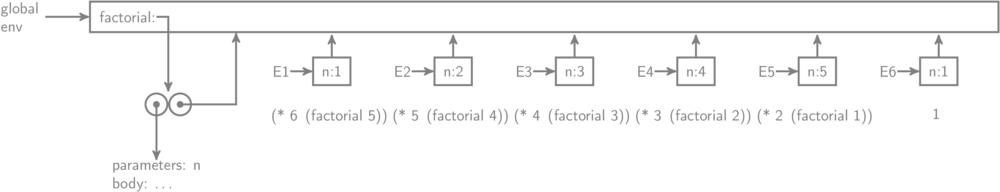
\includegraphics[width=.9\linewidth]{exercise-3-9-part-1.png}
\end{center}


Let us draw the environment number 2.


\lstset{numbers=left,frame=single,language=[LaTeX]TeX,label=org948427c,caption= ,captionpos=b}
\begin{lstlisting}
\begin{tikzpicture}[inner sep=0mm,>=stealth',very thick,color=black!50,
     font=\sffamily,pics/two dots/.style={code={
     \node [draw,minimum size=5mm,circle,colored tokens={black!50}]
     (#1-left) {};
    \node [draw,minimum size=5mm,circle,colored tokens={black!50},
    right=0pt of #1-left]
        (#1-right) {};
    \node [rectangle, fit=(#1-left) (#1-right)] (#1){};
    }},
    every pin edge/.style={<-,very thick},
    box/.style={draw,rectangle,inner sep=#1},box/.default=2mm]

  \node (W1)   {factorial:};
  \node (fake1) [right=340mm of W1] {};
  \node (fact-iter) [above=1mm of W1] {fact-iter:};
%
  \node (g env) [box, fit=(W1) (fake1) (fact-iter),
  pin={[text width=1cm,pin distance=10mm]left:global env}]
  { };
  % factorial
  \path ([yshift=-20mm]W1.east)pic{two dots=w1fun}
    (w1fun) edge [<-, to path={|- (\tikztotarget)}] (W1.east);
  \node [below=of w1fun-left, align=left] {\ttfamily \noindent parameters:\vphantom{d}n \\ body: \dots}
    edge [<-] (w1fun-left.center);
  \draw[->] (w1fun-right.center) -| ([xshift=3mm] w1fun-right.east |- g env.south);

  % fact-iter
\path coordinate[base right=22mm of w1fun.east] (aux)
    (aux) pic{two dots=fact-iter-fun}
    (fact-iter-fun) edge [<-, to path={|- (\tikztotarget)}] (fact-iter.east);
  \node [below=of fact-iter-fun-left, align=left,node font=\ttfamily] {
     parameters:product,\\
     \phantom{parameters:}counter,\\
     \phantom{parameters:}max-count \\ body: \dots}
    edge [<-] (fact-iter-fun-left.center);
  \draw[->] (fact-iter-fun-right.center) -| ([xshift=3mm] fact-iter-fun-right.east |- g env.south);

\path (g env.south west) -- (g env.south east)
\foreach \idx in {1,...,6}
{

  node [pos=2.6/7.5+\idx/11] (fake2-\idx)  {}
  node (E\idx-env) [below=5mm of fake2-\idx,box,
    pin={[pin distance=5mm]left:E\idx}, align=left] {
        counter:\idx\\
        product:\pgfmathparse{int(factorial(\idx-1))}\pgfmathresult \\
        max-count:6}
    edge [->] (fake2-\idx)

  node (E\idx-code) [below=5mm of E\idx-env, align=left]{
       (fact-iter\\
        (* counter product) \\
       (+ counter 1)  \\
       max-count)
    }
}
node [pos=2.6/7.5+7/11] (fake2-7) {}
node (E7-env) [below=5mm of fake2-7,box,
    pin={[pin distance=5mm]left:E7},align=left]
    {counter:7\\
     product:\pgfmathparse{int(factorial(7-1))}\pgfmathresult \\
     max-count:6
    }
    edge [->] (fake2-7)
node (E7-code) [below=5mm of E7-env, align=center]{
       720
    }
node [pos=2.0/7.5] (fake2-0) {}
node (E0-env) [below=5mm of fake2-0, box,
    pin={[pin distance=5mm]left:E0},align=left]
    {n:6}
    edge [->] (fake2-0)
node (E0-code) [below=5mm of E0-env, align=left]{
  (fact-iter 1 1 n)}
;

\end{tikzpicture}
\end{lstlisting}

\begin{center}
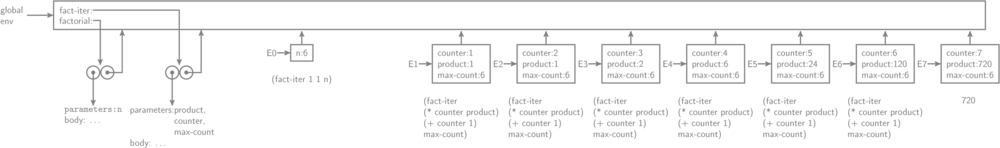
\includegraphics[width=.9\linewidth]{exercise-3-9-part-2.png}
\end{center}

These pictures would have never happened unless generous people from
\TeX{} StackExchange had helped.

\begin{itemize}
\item \url{https://tex.stackexchange.com/questions/515909/how-to-make-this-tikz-picture-more-idiomatic-environment-diagram/515913}
\item \url{https://tex.stackexchange.com/questions/516560/how-to-place-evenly-spaced-nodes-in-tikz-from-node1-to-node2}
\item \url{https://tex.stackexchange.com/questions/517061/how-to-debug-token-positions-in-petri-nets-in-tikz}
\item \url{https://tex.stackexchange.com/questions/517217/how-is-text-indented-and-glued-within-tikz-node-contents}
\end{itemize}

I feel that these diagrams are already quite cluttered, so I am
implicitly expanding \texttt{if} forms in the "code" blocks. I am also
ignoring top level commands and I am not drawing arrows when function
calls occur.\footnote{This exercise took me about 40 hours.}
\end{document}